%!TeX root=../tese.tex
%("dica" para o editor de texto: este arquivo é parte de um documento maior)
% para saber mais: https://tex.stackexchange.com/q/78101

\chapter{Results and experiments}
\label{results}

In this chapter we will describe the experiments we performed to compare the different building blocks for our model that we described in Chapter~\ref{chap:models}. To better understand the options available to build the best model possible, we begin by analyzing the proposed embeddings, first we compare the transformer based embeddings and then add GloVe to the analysis. With the ``best'' embedding selected we compare both proposed architectures and then lastly we train our definitive model based on the results of the previous experiments.





\section{Comparing transformer based embeddings}

To compare the transformer embeddings, we trained 7 pointer networks to compute the loss and accuracy graphs for these models in the validation and training datasets. In general, after the fourth epoch of training we began to see signs of overfitting in all of our models so here we only present training results up to the fourth epoch. In Fig~\ref{7loss} we can see the L1 loss plots of training and validation. In both cases ``paraphrase-albert-small-v2''  performed significantly worse than other models at all times. The best performing model isn't as clean cut as the worst but ``distiluse-base-multilingual-cased-v1'' --- or dbmc1 as we will call it from now on --- was able to attain the lowest validation loss at the third epoch.


\begin{table}[]
\begin{tabular}{lllll}
\multicolumn{1}{l|}{Embedding}                             & Acc train & Acc val & Loss train & Loss val \\ \hline
\multicolumn{1}{l|}{distiluse-base-multilingual-cased-v1}  & 0.7296    & 0.7263  & 5.485      & 6.423    \\
\multicolumn{1}{l|}{all-mpnet-base-v2}                     & 0.7215    & 0.7172  & 5.596      & 6.407    \\
\multicolumn{1}{l|}{all-distilroberta-v1}                  & 0.724     & 0.7178  & 5.554      & 6.442    \\
\multicolumn{1}{l|}{all-MiniLM-L12-v2}                     & 0.7234    & 0.7121  & 5.549      & 6.494    \\
\multicolumn{1}{l|}{paraphrase-albert-small-v2}            & 0.709     & 0.6961  & 5.747      & 6.559    \\
\multicolumn{1}{l|}{paraphrase-multilingual-MiniLM-L12-v2} & 0.7242    & 0.7102  & 5.546      & 6.496    \\
\multicolumn{1}{l|}{paraphrase-MiniLM-L3-v2}               & 0.7245    & 0.714   & 5.51       & 6.449    \\
\multicolumn{1}{l|}{distiluse-base-multilingual-cased-v2}  & 0.7271    & 0.7144  & 5.528      & 6.437
\end{tabular}
\caption{Accuracy and Loss of the final epoch for the eight different transformer based embeddings. Amongst the eight models ``distiluse-base-multilingual-cased-v2'' achieved the lowest loss validation score at the third epoch with a loss value of 6.334 followed by dbmc1 with a loss validation of 6.374 also at the third epoch.}
\label{table:8}
\end{table}


Alongside the L1 loss we recorded the jaccard binary accuracy score of the predictions at each epoch, which can be seen in Fig.~\ref{7acc} as the train and validation accuracy.
Once again ``paraphrase-albert-small-v2'' was the worst performing model and dbmc1 was the best performing model. 


\begin{figure}[!ht]
\centerline{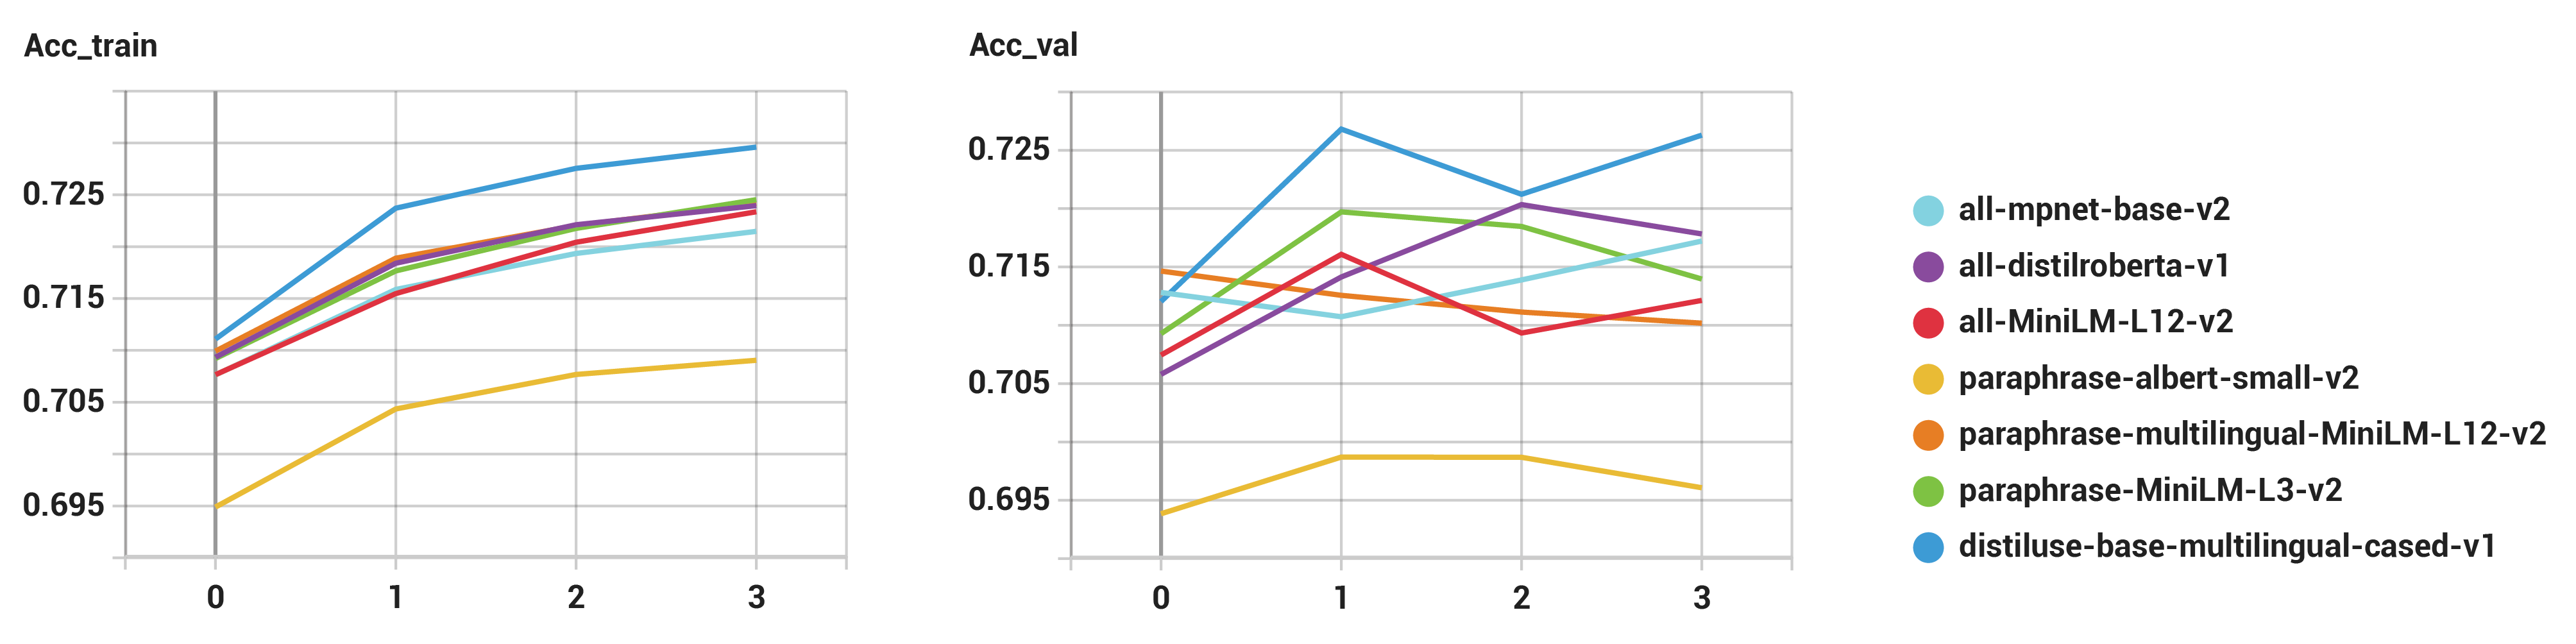
\includegraphics[width=1.1\textwidth]{figuras/7embeddings_transformer_-ACC.png}   }
\caption{Train and validation binary accuracy score of the seven transformer based models.}
\label{7acc}
\end{figure}

\begin{figure}[!ht]
\centerline{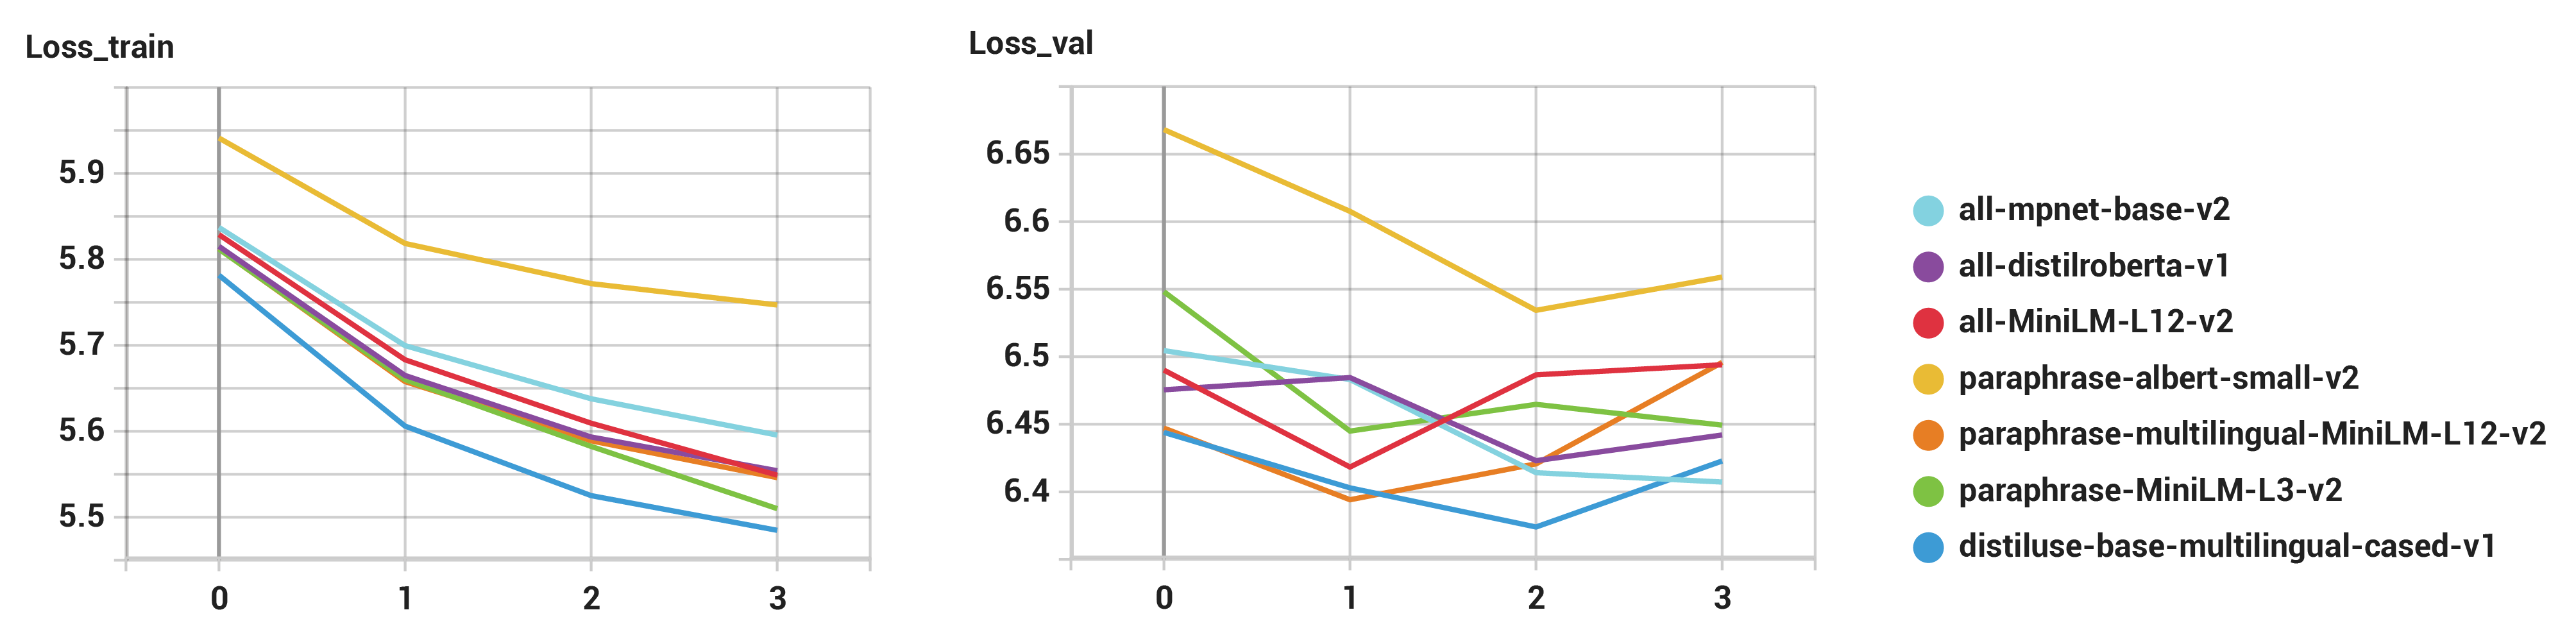
\includegraphics[width=1.1\textwidth]{figuras/7embeddings_transformer_-Loss.png}   }
\caption{L1 training and validation loss of the seven transformer based models. }
\label{7loss}
\end{figure}

Due to the unexpectedly great performance of dbmc1 we decided to test ``distiluse-base-multilingual-cased-v2'' to validate if we were correct in our initial assumption that including another 35 languages in the training process wouldn't  bring us much benefit. In Fig.~\ref{multilingual_acc} and Fig.~\ref{multilingual_loss} we can see the results of their comparison.
Against our expectations, ``distiluse-base-multilingual-cased-v2'' was capable of obtaining a lower validation  loss than its predecessor at the third epoch, however its accuracy was consistently lower in both training and validation. Since accuracy should better translate into real world performance we will be keeping dbmc1 as the best performing model overall with a validation accuracy of 72.63\%. Table~\ref{table:8} compiles the loss and accuracy results of these models.

\begin{figure}[!ht]
\centerline{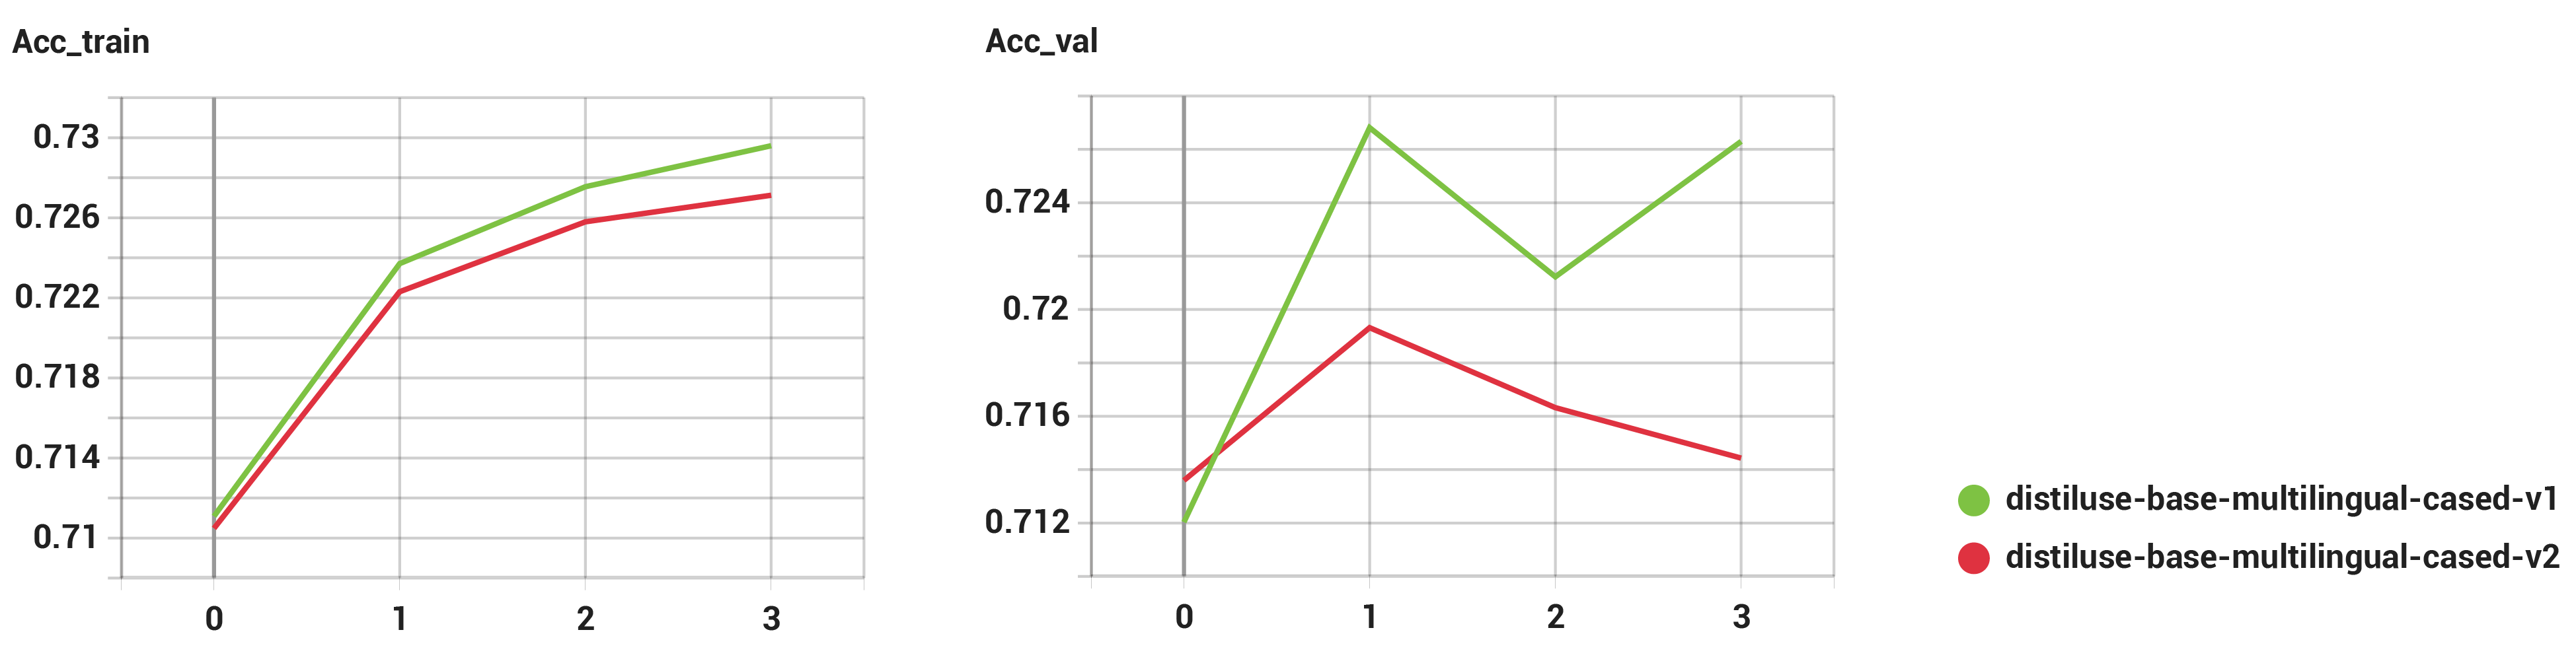
\includegraphics[width=1.1\textwidth]{figuras/multilingual_1vs2_-Acc.png}   }
\caption{Comparison of accuracy in validation and train sets between models dbmc1 and ``distiluse-base-multilingual-cased-v2''.}
\label{multilingual_acc}
\end{figure}


\begin{figure}[!ht]
\centerline{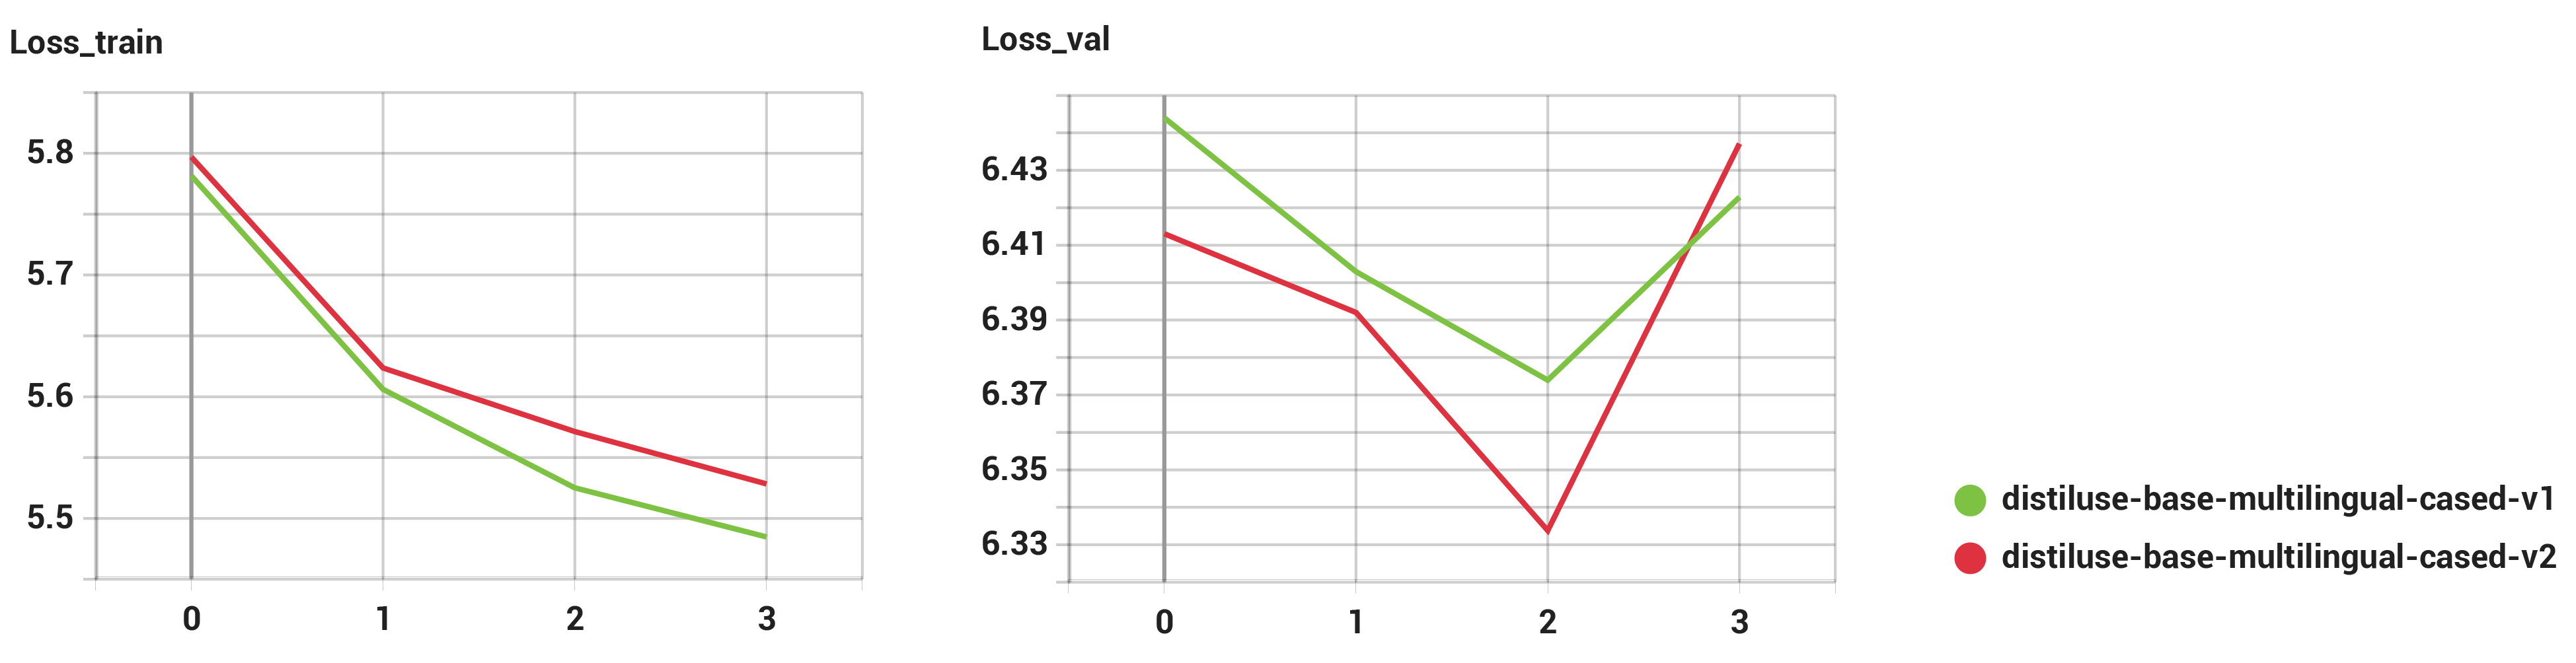
\includegraphics[width=1.1\textwidth]{figuras/multilingual_1vs2_-Loss.png}   }
\caption{Comparison of loss in validation and train sets between models dbmc1 and ``distiluse-base-multilingual-cased-v2''.}
\label{multilingual_loss}
\end{figure}


\section{Adding GloVe to the comparison}


In Fig.~\ref{glove_loss} and Fig.~\ref{glove_acc} we compare the pointer network models trained with transformer based embeddings with their GloVe counterpart, which was the best performing model we obtained through Optuna in section \ref{optuna}. In the interest of clarity we decided to omit some of the  transformer models from the graphs to avoid clutter, we plot only the best performing transformer-based model and the two other that are adjacent in performance to the GloVe-based model. The graph makes it clear that the GloVe-based model performed consistently worse than all the transformer-based models, except for model ``paraphrase-albert-small-v2'' which was the worst performing one. Table~\ref{table:glove} compiles the final accuracy and loss of all of the presented transformer models and the GloVe model.

% Please add the following required packages to your document preamble:
% \usepackage[table,xcdraw]{xcolor}
% If you use beamer only pass "xcolor=table" option, i.e. \documentclass[xcolor=table]{beamer}
\begin{table}[]
\begin{tabular}{l|llll}
Embedding                             & Acc train & Acc val & Loss train & Loss val \\ \hline
distiluse-base-multilingual-cased-v1  & 0.7296    & 0.7263  & 5.485      & 6.423    \\
all-mpnet-base-v2                     & 0.7215    & 0.7172  & 5.596      & 6.407    \\
all-distilroberta-v1                  & 0.724     & 0.7178  & 5.554      & 6.442    \\
all-MiniLM-L12-v2                     & 0.7234    & 0.7121  & 5.549      & 6.494    \\
paraphrase-albert-small-v2            & 0.709     & 0.6961  & 5.747      & 6.559    \\
paraphrase-multilingual-MiniLM-L12-v2 & 0.7242    & 0.7102  & 5.546      & 6.496    \\
paraphrase-MiniLM-L3-v2               & 0.7245    & 0.714   & 5.51       & 6.449    \\
distiluse-base-multilingual-cased-v2  & 0.7271    & 0.7144  & 5.528      & 6.437    \\
\rowcolor[HTML]{F9F5E9} 
glove.840B.300d                         & 0.7123    & 0.7046  & 5.64       & 6.447   
\end{tabular}
\caption{Accuracy and Loss of the final epoch for the eight different transformer based embeddings and the GloVe based embedding.}
\label{table:glove}
\end{table}


\begin{figure}[!ht]
\centerline{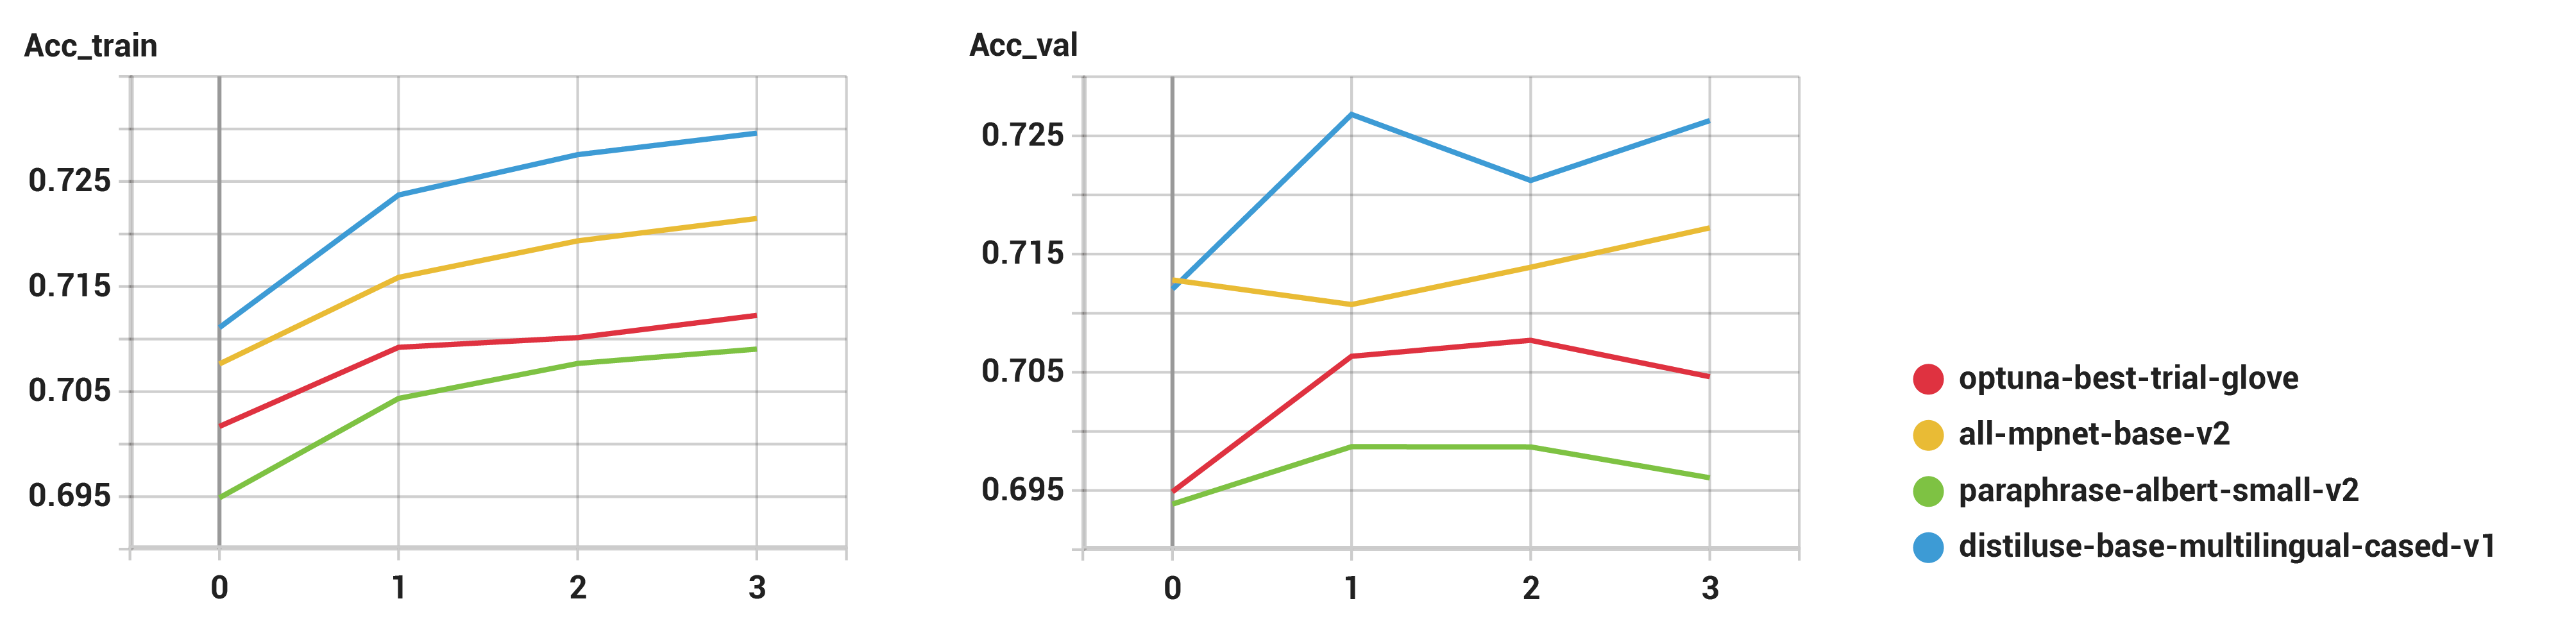
\includegraphics[width=1.1\textwidth]{figuras/glove_vs_transformer_-ACC.png}   }
\caption{Plots comparing the training and validation accuracy of four pointer networks trained with a GloVe embedding and 3 other transformer based embedding.}
\label{glove_acc}
\end{figure}

\begin{figure}[!ht]
\centerline{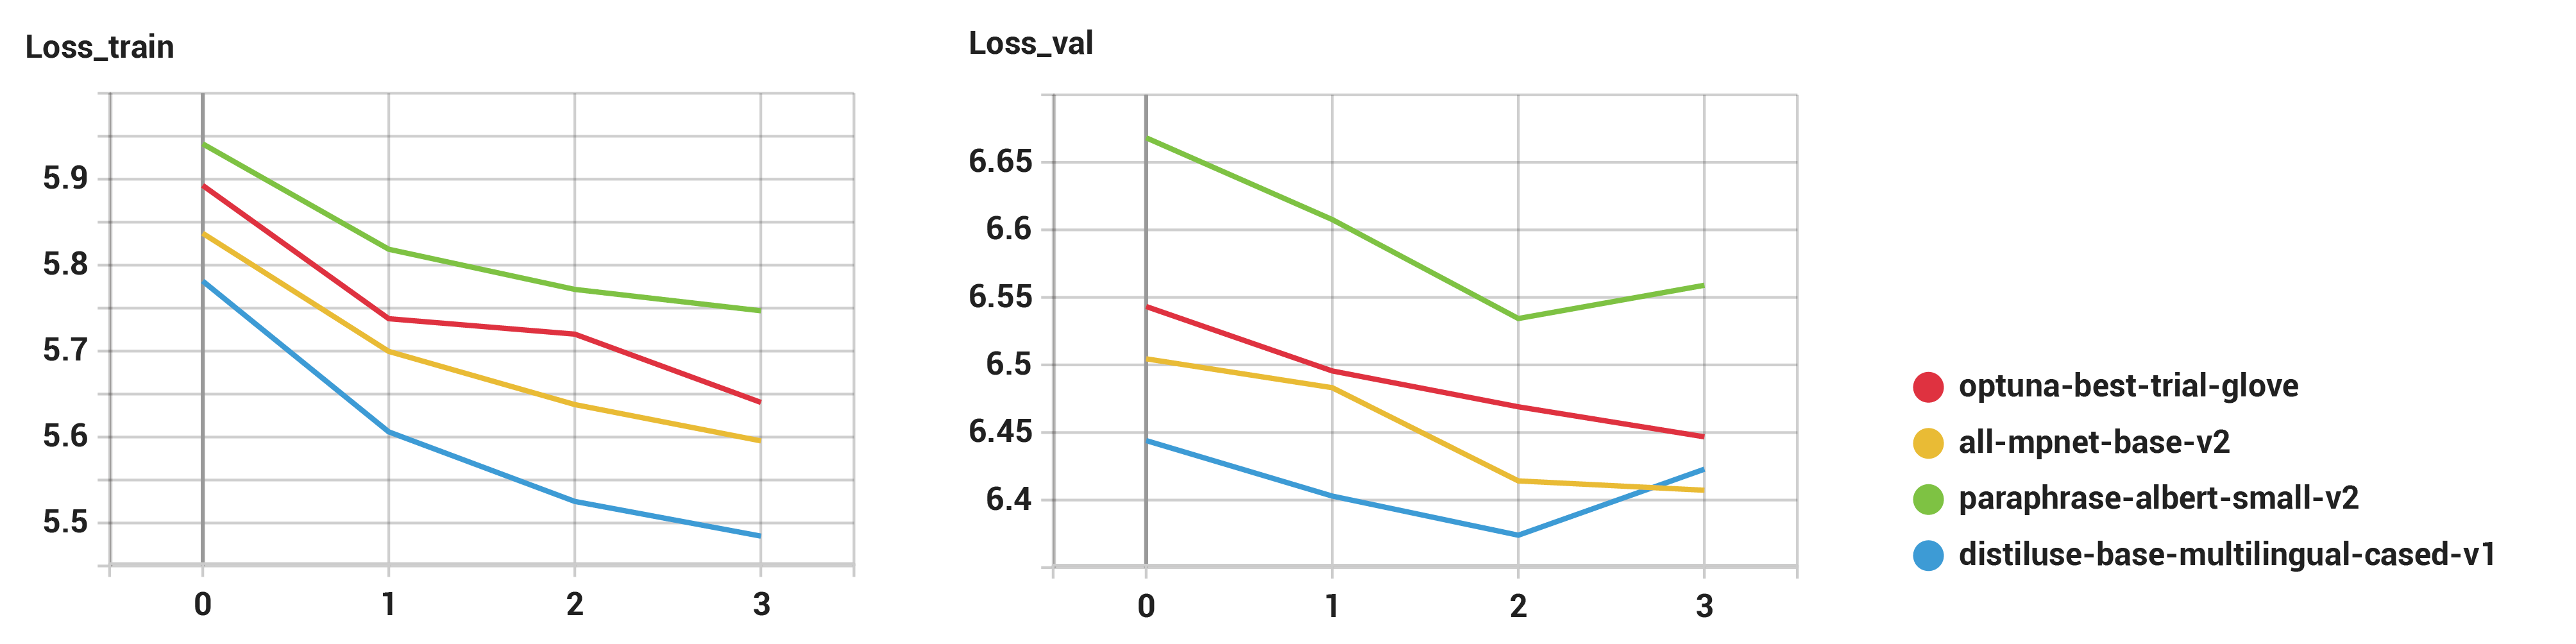
\includegraphics[width=1.1\textwidth]{figuras/glove_vs_transformer_-Loss.png}} 
\caption{Plots comparing the training and validation loss of four pointer networks trained with a GloVe embedding and 3 other transformer based embedding.}
\label{glove_loss}
\end{figure}




\section{Comparing architectures}

 
In Fig.~\ref{arq_acc} and Fig.~\ref{arq_loss} we compare our two architectures, the pointer network and our so-called ``simple RNN''. We trained both models with the best performing embedding we found in previous sections, the dbmc1 embedding, and found that the Ptr-Net outperformed the simple RNN in all 4 metrics as can be seen in Table~\ref{table:arq}. 


\begin{figure}[!ht]
\centerline{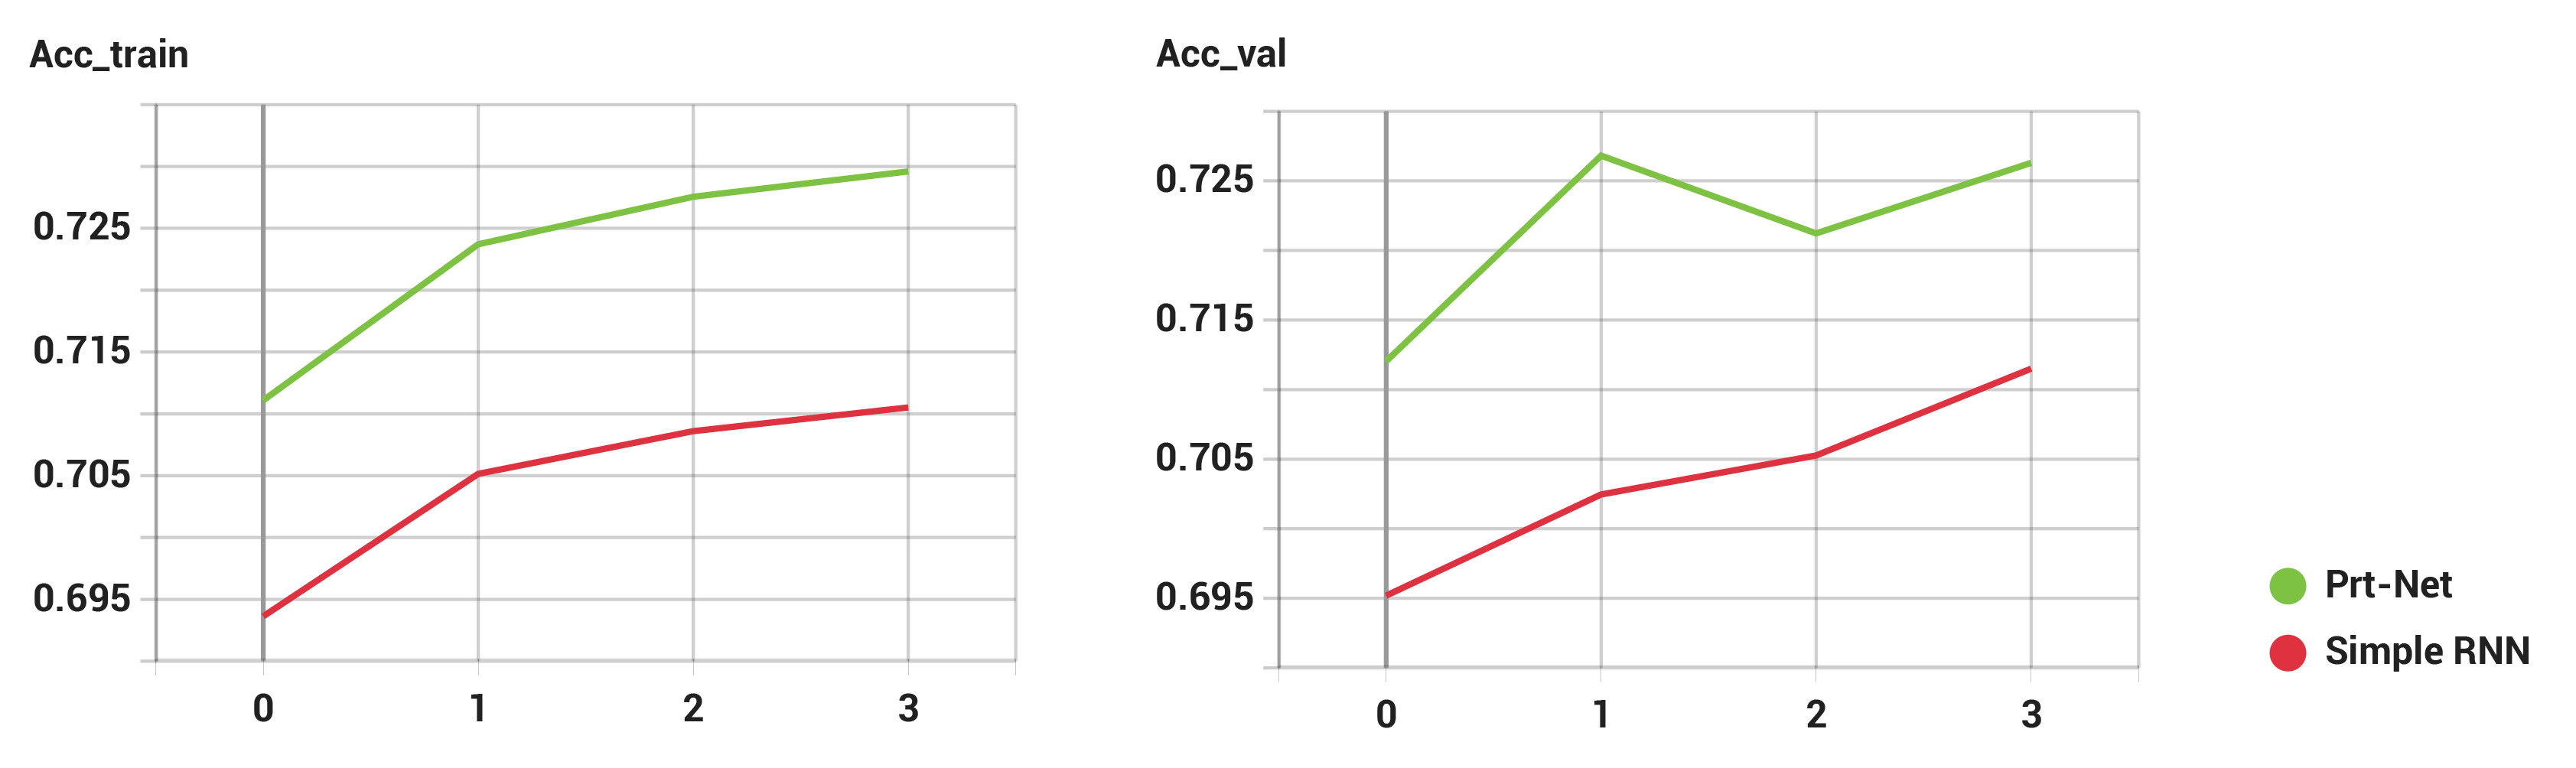
\includegraphics[width=1.1\textwidth]{figuras/arquiteturas_-ACC.png}   }
\caption{Plots comparing the training and validation accuracy of our two architectures trained with the  dbmc1 embedding.}
\label{arq_acc}
\end{figure}

\begin{figure}[!ht]
\centerline{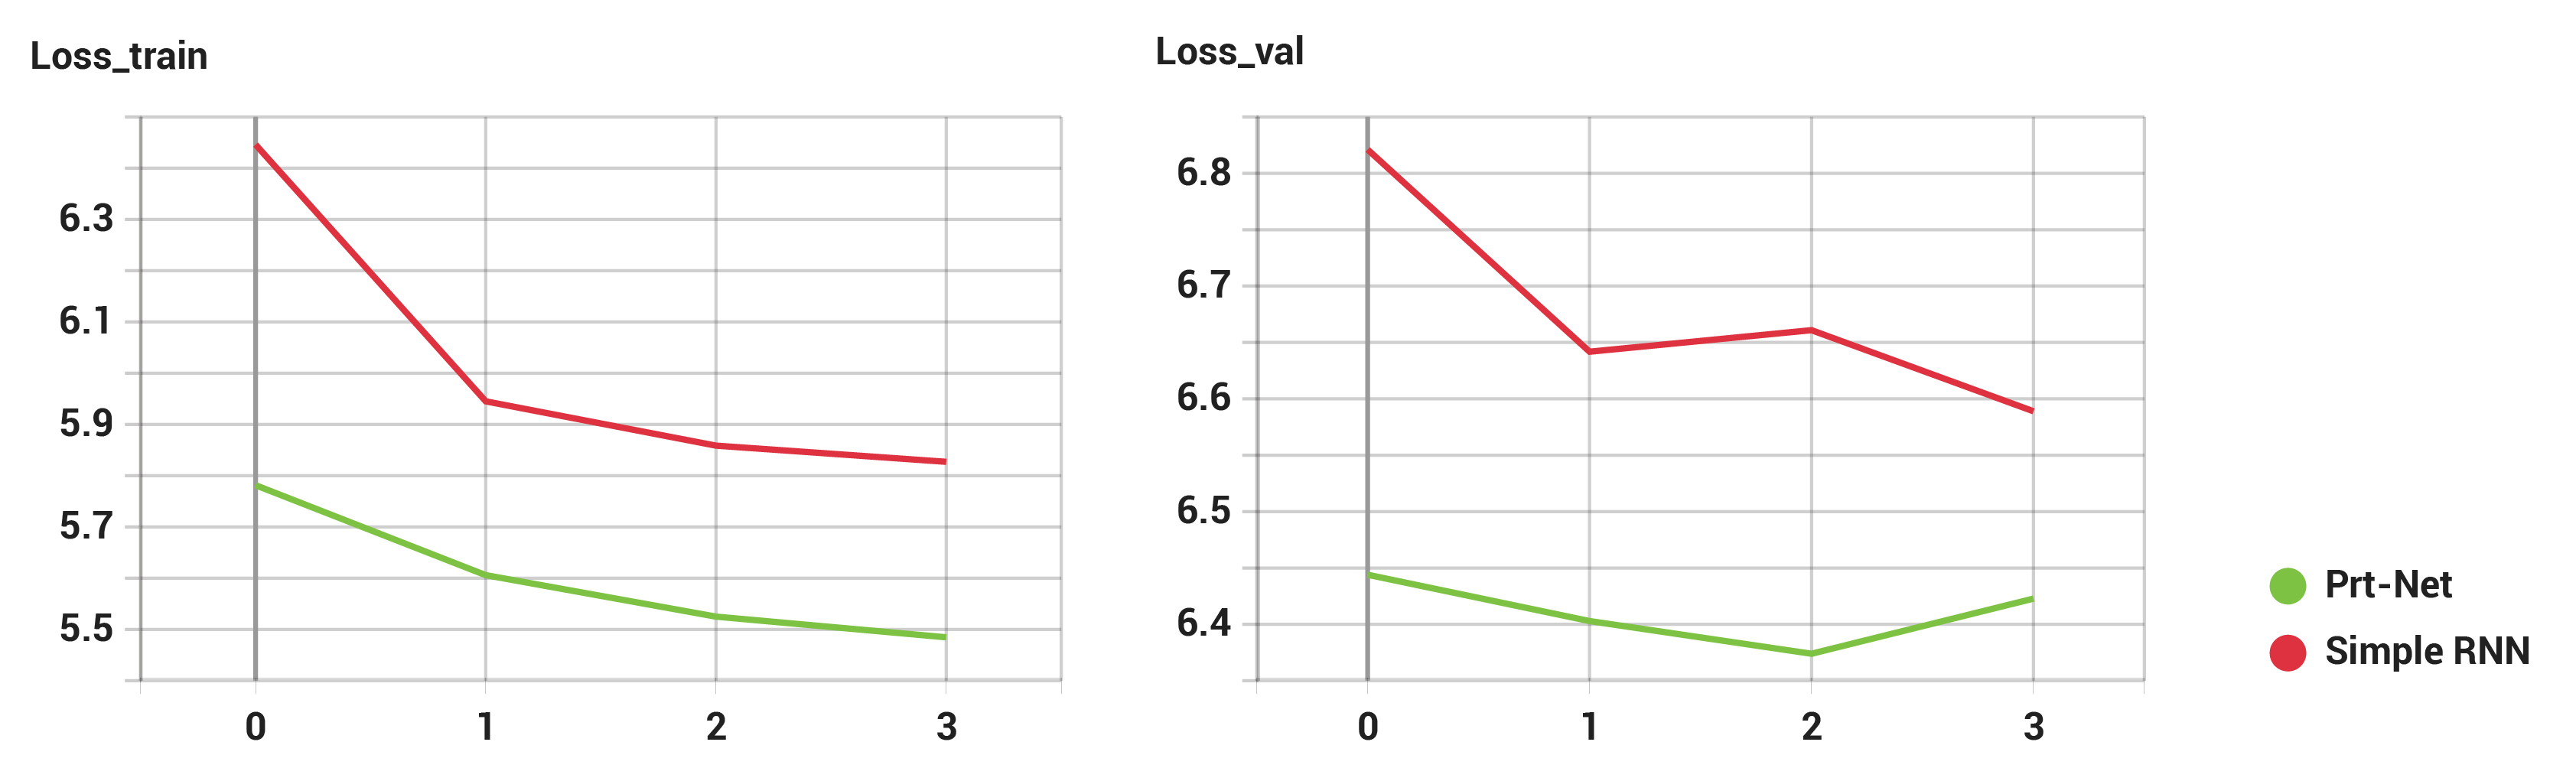
\includegraphics[width=1.1\textwidth]{figuras/arquiteturas_-Loss.png}   }
\caption{Plots comparing the training and validation loss of our two architectures trained with the dbmc1 embedding.}
\label{arq_loss}
\end{figure}

\begin{table}[]
\begin{tabular}{l|llll}
Architecture & Acc train & Acc val & Loss train & Loss val \\ \hline
Ptr-Net      & 0.7296    & 0.7263  & 5.485      & 6.423    \\
Simple RNN   & 0.7105    & 0.7115  & 5.827      & 6.589   
\end{tabular}
\caption{Table of the final (fourth epoch) loss and accuracy in the training and validation sets for our two different architectures.}
\label{table:arq}
\end{table}

\section{Best Model}

Taking into account all our previous findings we can conclude that the pointer network architecture combined, with the dbmc1 embedding and the hyperparameters found by Optuna form our best performing model, Fig.~\ref{fig:final_model} illustrates succinctly this final model.  In Fig.~\ref{best_acc} and Fig.~\ref{best_loss} we present the accuracy and loss plots for this model in the training and testing datasets and in Table~\ref{table:best} we compile its final accuracy and loss scores.


\begin{figure}[!ht]
\centerline{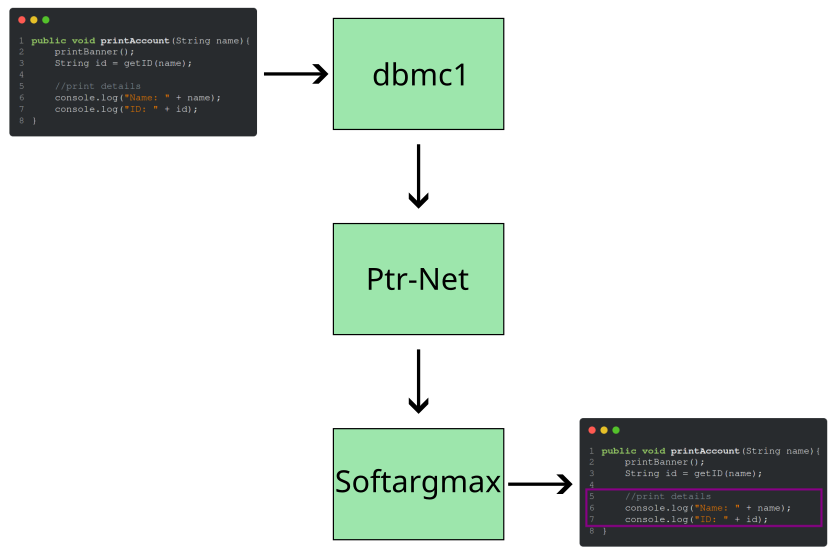
\includegraphics[width=1.1\textwidth]{figuras/final_model.png}   }
\caption{Illustration of our final and best performing model. As previously mentioned, the hyper-parameters were chosen based on our Optuna experiments.}
\label{fig:final_model}
\end{figure}

\begin{table}[]
\begin{tabular}{l|llll}
Architecture                                                                                                & Acc train & Acc test & Loss train & Loss test \\ \hline
\begin{tabular}[c]{@{}l@{}}Ptr-Net and distiluse-base-\\ multilingual-cased-v1 \\ (Best Model)\end{tabular} & 0.7274    & 0.7275   & 5.529      & 5.768    
\end{tabular}
\caption{Accuracy and loss of the final epoch in the training and test sets for the final model, trained with the Ptr-Net architecture and the dbmc1 embedding.}
\label{table:best}
\end{table}

\begin{figure}[!ht]
\centerline{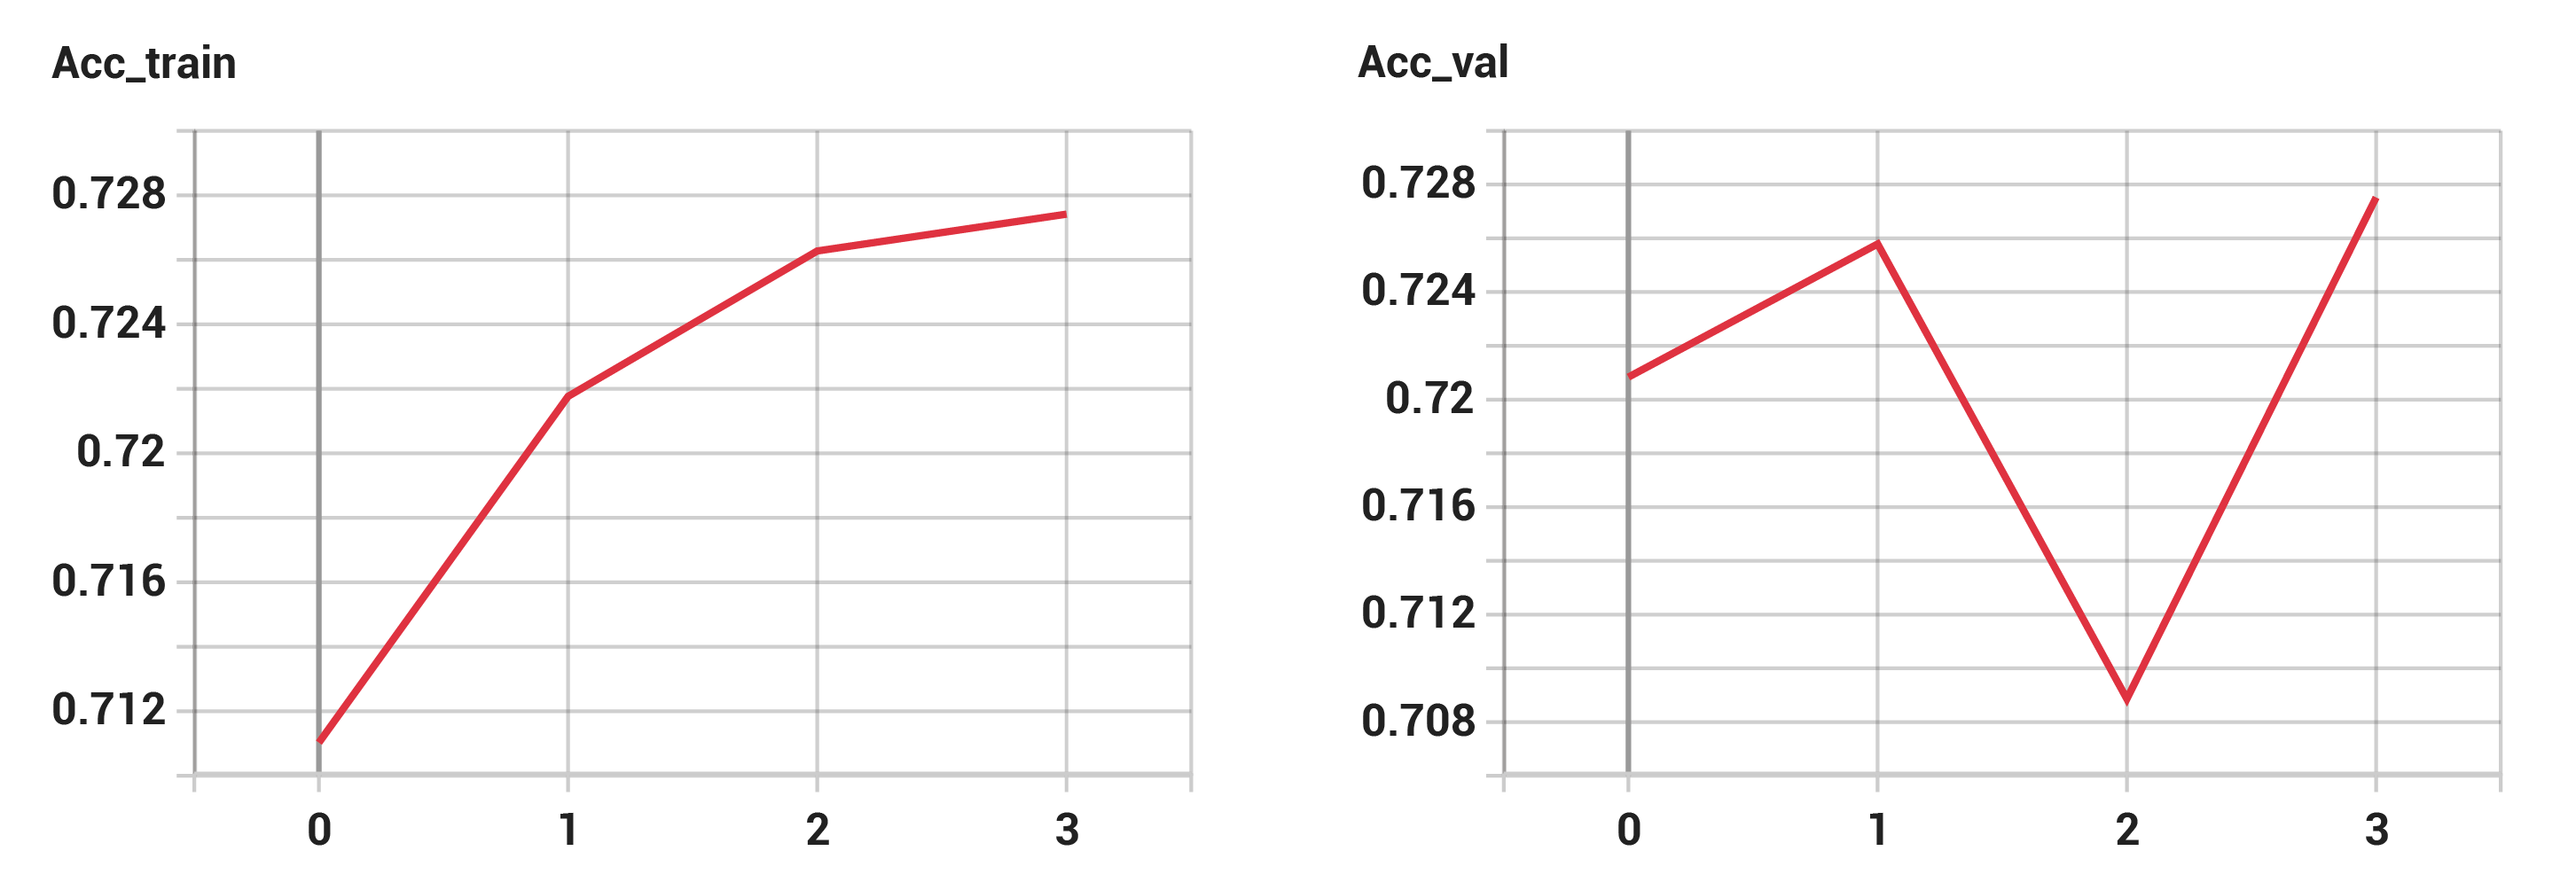
\includegraphics[width=1.1\textwidth]{figuras/best_model_-ACC.png}   }
\caption{Training and testing plots of accuracy of our best performing model in validation. Final accuracy value: 0.7275.}
\label{best_acc}
\end{figure}

\begin{figure}[!ht]
\centerline{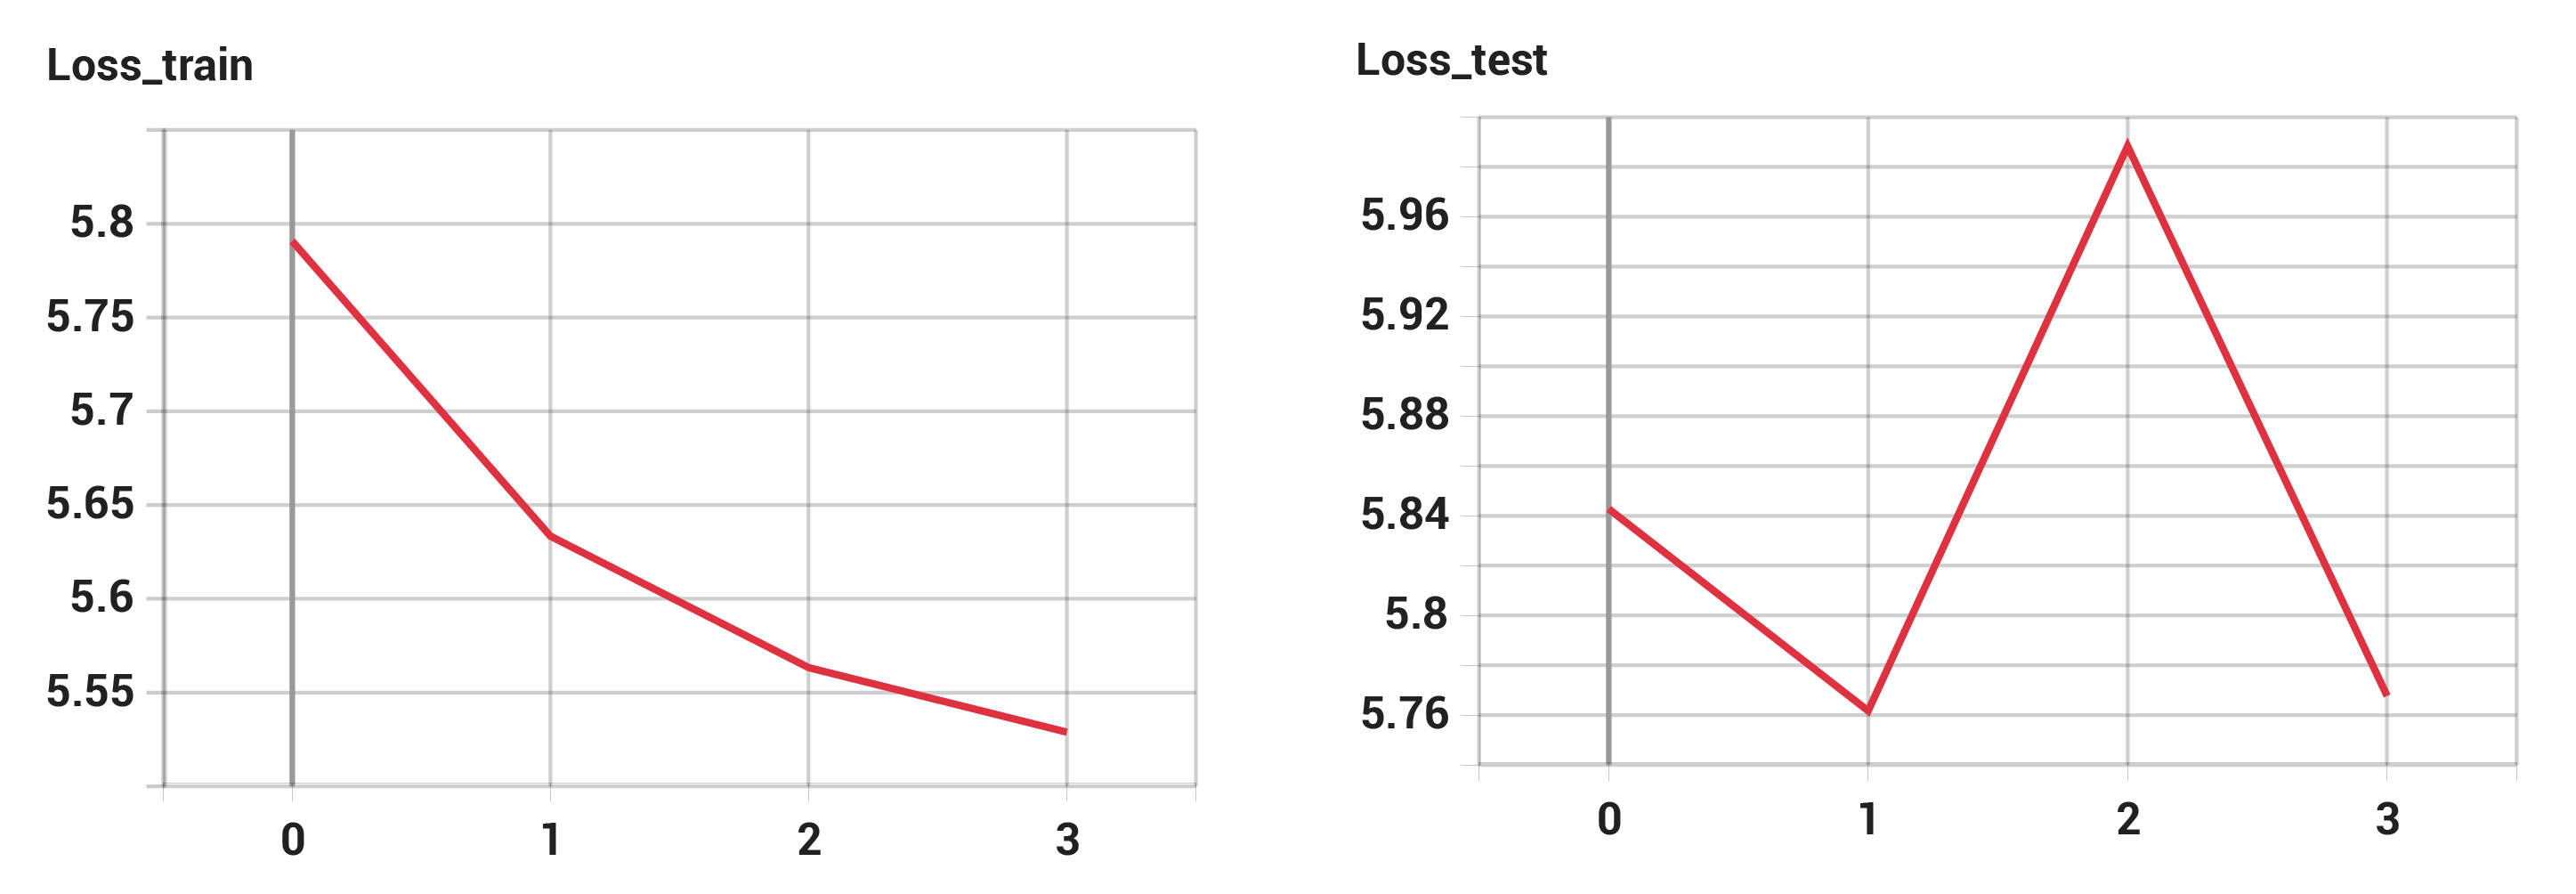
\includegraphics[width=0.8\textwidth]{figuras/best_model_-Loss.png}   }
\caption{Training and testing plots of loss of our best performing model in validation. Final loss value: 5.768.}
\label{best_loss}
\end{figure}


As an alternative, dbmc1 could be swapped by the GloVe embedding in the interest of speeding up inference time. Albeit when doing a single prediction the inference time of dbmc1 is greater than that of GloVe it is not as significant of an increase as when training the models where the process takes multiple days for each transformer based embedding over the few hours of GloVe based models. This decision should be taken case by case, for some applications keeping the inference time as small as possible may be more important than the 0.01\% performance gain of using dbmc1.



Whatever choice is made in a hypothetical deployment aside, we believe this model achieved the objectives we set. In conjunction with a language server it can easily execute function extraction refactorings and in conjunction with a refactoring opportunity detector these 3 components together could become a IDE plugin that automates the entirety of the function extraction process.

\subsection{Publication of results}

The student is preparing to submit these results as a scientific paper to a peer reviewed journal.


